\chapter{Marco Conceptual}
\label{chap:background}

\section{Codificaci\'on de Video}
Un problema de los videos sin compresi\'on (RAW) ha sido el almacenamiento y la transmisi\'on, debido al gran n\'umero de bits que contienen. Por esta raz\'on se requiere el uso de t\'ecnicas de compresi\'on para reducir el n\'umero de bits que representan el video. La codificaci\'on de video toma ventaja de tres tipos de redundancias  presentes en un video \cite{motion}:
\begin{itemize}
    \item \textbf{Redundancia estad\'istica:} se refiere a la alta correlaci\'on espacial entre pixeles en un frame y la correlaci\'on temporal entre pixeles co-localizados en frames consecutivos.
    \item \textbf{Redundancia psicovisual:} debido a las limitaciones y caracter\'isticas del sistema visual humano se puede eliminar informaci\'on que no se distingue.
    \item \textbf{Redundancia de C\'odigo:} se produce por la repetici\'on de s\'imbolos que representan la informaci\'on de video.
\end{itemize}

Los est\'andares de codificaci\'on implementan un conjunto de herramientas para explotar estas redundancias de un video. La figura \ref{codec} presenta un diagrama de bloques de un est\'andar de codificaci\'on de video, el cual tiene dos m\'odulos principales, el codificador y el decodificador.
	
\begin{figure}[!h]
\centering
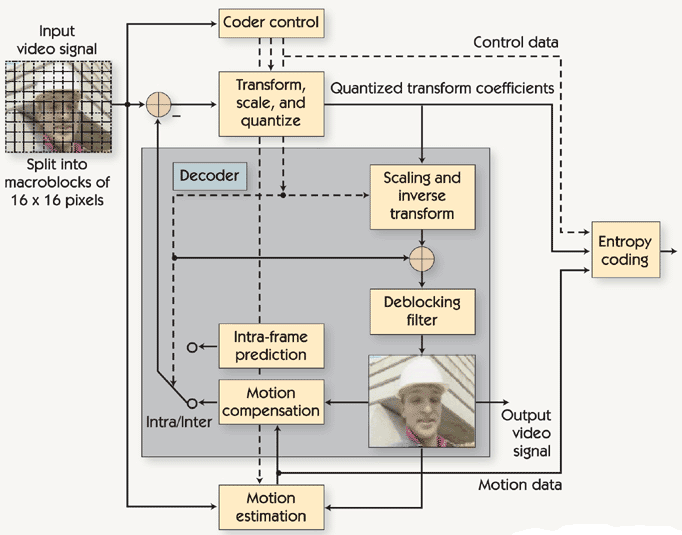
\includegraphics[width=0.6\textwidth]{images/codec.png}
\caption[Diagrama de Bloques de un est\'andar de codificaci\'on de video]{Diagrama de Bloques de un est\'andar de codificaci\'on de video
\scriptsize{\textbf{Fuente:} \url{http://www.eetimes.com/document.asp?doc_id=1272639}}}
\label{codec}
\end{figure}

Los codificacores de video consiste de tres elementos principales, los cuales explotan cada una de las redundancias:
\begin{itemize}
	\item El \textbf{predictor} que realiza una predicci\'on intra-frame para explotar la correlaci\'on espacial y una predicci\'on inter-frame para explotar la correlaci\'on temporal. 
	\item El \textbf{cuantizador} reduce la exactitud de las representaciones del predictor mediante un criterio de fidelidad para eliminar la redundancia psicovisual.
	\item La \textbf{codificaci\'on de entrop\'ia} reduce el n\'umero de s\'imbolos necesarios para representar el video aprovechando la similaridad de los s\'imbolos resultantes de la cuantizaci\'on.
\end{itemize}

Los codificadores realizan el proceso inverso de cada uno de los elementos para reconstruir la informaci\'on codificada. En el proceso de reconstrucci\'on se presenta p\'erdida de la informaci\'on debido a la eliminaci\'on o tranformaci\'on de la informaci\'on original en el codificador.

\section{Compressive Sensing}

La p\'erdida de informaci\'on en la codificaci\'on de video esta relacionada a dos suposiciones: la primera es la imperfecci\'on del HVS (sensitividad) y la segunda est\'a relacionada a propiedades espec\'ificas de la se\~nal en cierto dominio transformado. El objetivo de \textit{compressed sensing} (CS) es reconstuir una se\~nal usando un peque\~no conjunto de muestras de la se\~nal \cite{compressive}. Uno de los principales requerimientos que se deben satisfacer para aplicar t\'ecnicas de CS es la representaci\'on dispersa. 

\subsection{Representaci\'on dispersa}

Consideramos una se\~nal $\boldsymbol{x} \in \mathbb{R}^N$. Dada una matriz de base ortonormal $\boldsymbol{B} \in \mathbb{R}^{N \times N}$, donde sus columnas son lo elementos base $ \{\boldsymbol{b}_i\}_{i=1}^N$, $\boldsymbol{x}$ puede ser representada en t\'erminos de este base como:
\begin{center}
\begin{equation}
\boldsymbol{x}=\sum \limits_{i=1}^{N} \boldsymbol{\alpha}_i \boldsymbol{b}_i
\end{equation}
\end{center}
donde $\boldsymbol{\alpha}$ es un vector de coeficientes  y $\boldsymbol{b}_i$ son los \'atomos del diccionario \cite{sparsity}. Estos coeficientes son dados por $\alpha_i = \boldsymbol{x} \boldsymbol{b}_i^T$. Si el n\'umero de coeficientes diferentes a cero en $\boldsymbol{x}$ es $K\ll N$, la base $\boldsymbol{b}$ proporciona una representaci\'on K-dispersa de $\boldsymbol{x}$. La representaci\'on dispersa de un vector $\boldsymbol{\alpha}$ est\'a relacionada con $||\alpha||_0 = K$ donde $||.||_p$ indica la norma $\ell_p$ definida como:
\begin{equation}
||\boldsymbol{\alpha}||_p = \left(\sum\limits_{i=1}^{n} |\alpha_i|^p \right)^\frac{1}{p}
\end{equation}
y $||\alpha||_0$ es la norma $\ell_0$, la cual indica el n\'umero de elementos que son cero en el vector, y esta definida como
\begin{equation}
||\boldsymbol{\alpha}||_0 = \lim_{p \to 0} ||\alpha||_p^p=\lim_{p \to 0} \sum_i |\alpha_i|^p
\end{equation} 

Generalmente, las se\~nales del mundo real no son exactamente dispersas en una base ortogonal, en su lugar son \emph{compresibles}. Una se\~nal es compresible si las magnitudes de sus coeficientes, ordenados en un orden decreciente, presentan decaimiento de la ley de poder, tal que:
\begin{equation}
|\alpha|_{(n)} \leq C n^{-s}\;,\quad s=1,2 \ldots
\end{equation}

donde $|\alpha|_{(n)}$ es la $n$-ava entrada m\'as grande de  $\alpha$ y $C$ es una constante. Debido a que las magnitudes de los coeficientes decaen rapidamente, un n\'umero peque\~no de \'atomos $K\ll N$ de $\boldsymbol{B}$ puede proporcionar una aproximaci\'on de $\boldsymbol{x}$. El error entre la se\~nal original y su aproximaci\'on esta dada por:
\begin{equation}
||\boldsymbol{x}_L - \boldsymbol{x}||_2 \leq CL^{-(s-\frac{1}{2})}
\end{equation}
donde $L$ es el t\'ermino de la combinaci\'on lineal de elementos que mejor aproxima a $\boldsymbol{x}$.  

\subsection{Muestreo Incoherente}

Un conjunto de muestras aleatorias seleccionadas desde la se\~nal $\boldsymbol{x}$ son usadas para construir una matriz $\boldsymbol{\phi} \in \mathbb{R}^{M \times N}$ tal que:
\begin{equation}
\boldsymbol{y} = \boldsymbol{\phi x}
\end{equation}
donde $\boldsymbol{y}$ es un vector $M\times 1$ de medidas compresivas.  Para reconstruir $\boldsymbol{x}$ desde $\boldsymbol{y}$, $\boldsymbol{x}$ debe ser disperso en un dominio transformado (definido por la matriz de base ortogonal $\boldsymbol{B}$), tal que:
\begin{equation}
\boldsymbol{y}=\boldsymbol{\phi B \alpha}= \boldsymbol{D\alpha}
\end{equation}
La incoherencia est\'a relacionada con la propiedad de la se\~nales que tiene representaci\'on dispersa en un dominio transformado $\boldsymbol{\psi}$, las cuales deben ser densas en el dominio donde se realiz\'o la adquisici\'on \cite{compressive}. La coherencia entre una base sensada $\boldsymbol{\phi}$  y una base de representaci\'on $\boldsymbol{\psi}$ est\'a dada por: 

\begin{equation}
\mu(\boldsymbol{\phi},\boldsymbol{B})= \sqrt{N} \max_{1 \leq j, j \leq N} | \boldsymbol{\varphi}_i,\boldsymbol{b}_j|, \quad 1\leq \mu(\boldsymbol{\phi},\boldsymbol{B}) \sqrt{N}
\end{equation}
Si la coherencia es baja, un n\'umero de muestras aleatorias para reconstruir la se\~nal es peque\~no porque cada fila de $\boldsymbol{\phi}$ se extiende en el dominio $\boldsymbol{B}$.

\subsection{Propiedad Isom\'etrica Restringida (RIP)}

Esta propiedad ayuda a determinar si la matriz $\boldsymbol{D}$ es  buena para realizar CS. Una matriz $\boldsymbol{D}$ satisface la RIP, si por cada $K = 1,2, \ldots, N$, la constante isom\'etrica $\delta_K$ de la matriz $\boldsymbol{D}$ es el n\'umero m\'as peque\~no, tal que: 
\begin{equation}
(1-\delta_K)||\boldsymbol{x}||_2^2 \leq ||\boldsymbol{Dx}||^2_2 \leq (1+\delta_K)||\boldsymbol{x}||^2_2
\end{equation}
para todos los vectores K-dispersos de $\boldsymbol{x}$. Est\'a propiedad es equivalente a decir que todos los $K$ subconjuntos tomados de las columnas pertenecientes a $\boldsymbol{D}$ son casi ortogonales y los vectores K-dispersos no se encuentran en el espacio nulo de $\boldsymbol{D}$.

\subsection{Optimizaciones Num\'ericas}

Un sistema de ecuaciones lineales con una matriz $\boldsymbol{D} \in \mathbb{R}^{M \times N}$ representa un sistema de ecuaciones indeterminado que puede tener infinitas soluciones. El m\'etodo para resolver este sistema y hallar la representaci\'on dispersa de la se\~nal es encontrar la norma m\'inima mediante un proceso de optimizaci\'on, tal que: 
\begin{equation}
\min||\boldsymbol{\alpha^\prime}||_0 \quad \textrm{subject to} \; \boldsymbol{x} = \boldsymbol{D \alpha^\prime}
\end{equation}
Aunque solucionando este problema de optimizaci\'on se puede hallar directamente la representaci\'on dispersa, es un problema NP-Hard porque requiere una b\'usqueda combinatoria exhaustiva. En algunos casos, es usada la norma $\ell_1$ y $\ell_2$ para aproximar la soluci\'on dispersa. \\


El proceso de CS es resumido en la Figura \ref{fig:compressive}. Una vez es conseguida una soluci\'on dispersa, la se\~nal puede ser recosntruida en base a un vector con una gran cantidad de coeficientes igual a cero y un diccionario $\boldsymbol{D}=\boldsymbol{\phi B}$.
\begin{figure}[!h]
\centering
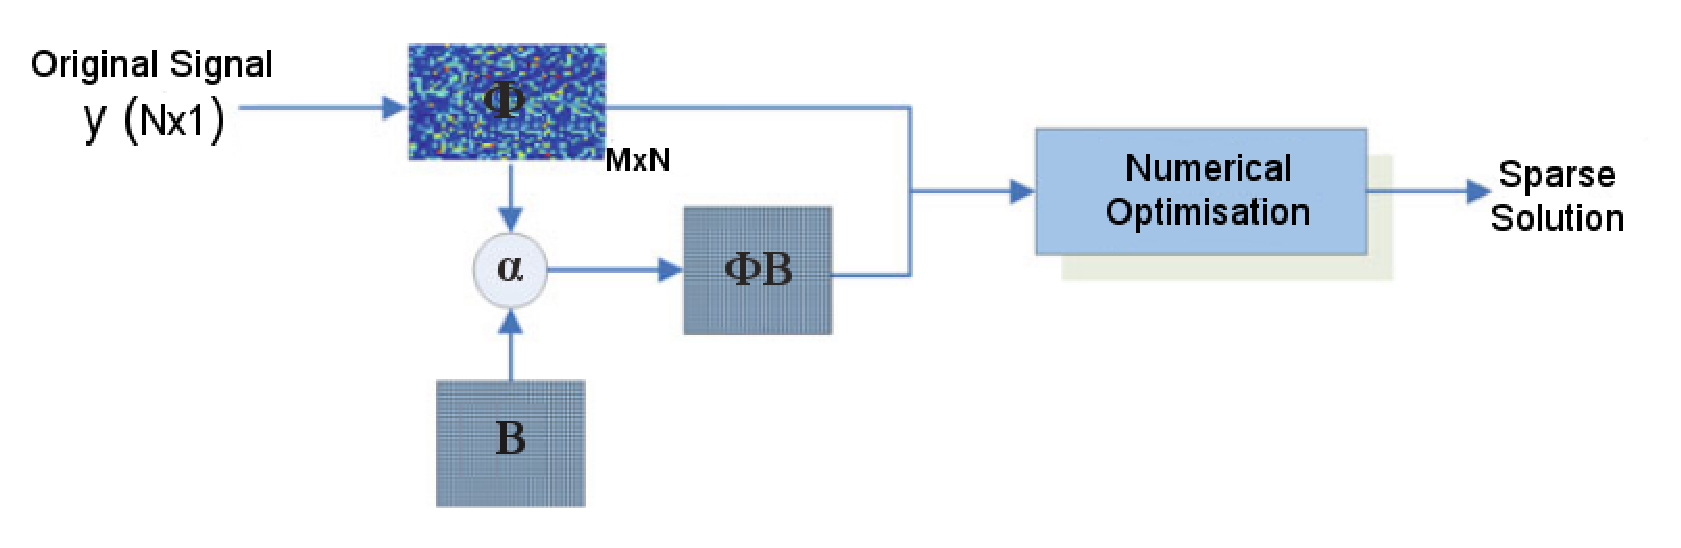
\includegraphics[width=\textwidth]{images/sparse.eps}
\caption[Proceso de \textit{Compressed sensing}]{Proceso de \textit{Compressed sensing} \cite{compressive}}
\label{fig:compressive}
\end{figure}











